\chapter{Contrasting effects of core intensity and organisation on the lifecycle and thin anvil extent of \acrshort{dcc}s} \label{chp:anvil_structure}

\section{Introduction}

Understanding how the structure of anvil clouds changes in response to changes in convective behaviour is vital to understanding climate feedbacks of \acrshort{dcc}s.
Around 50\% of cirrus clouds in the tropics originate from deep convection \citep{massie_distribution_2002, luo_characterizing_2004}.
While the optically thick portion of anvil clouds generally has a neutral effect on the \acrshort{toa} radiative balance, thin cirrus clouds have a strong warming effect \citep{berry_cloud_2014}.
As a result, changes in convective activity that result in a change in the size of the thin anvil coverage may have large climate feedbacks.

The change of anvil cloud area in response to warming (the iris effect \citep{lindzen_does_2001, bony_thermodynamic_2016}) is generally considered to have a cooling feedback in response to climate change.
However, it is the largest source of uncertainty in cloud--climate feedbacks, with around a third of models predicting a warming response \citep{sherwood_assessment_2020}.
To address this uncertainty, a better understanding of the links between convective processes and anvil properties, changes in anvil structure and the properties of ice clouds are required \citep{gasparini_opinion_2023}.

Assessing the extent of thin anvil cirrus is challenging due to the difficulties in observing these clouds using \acrshort{ir} radiometers.
The low emissivity of thin cirrus clouds means that observed \acrshort{bt} is dominated by radiances from the lower atmosphere and surface below.
\citet{protopapadaki_upper_2017} used cloud emissivity and cloud top pressure, rather than \acrshort{bt}, to detect convective cores, thick and thin anvil cirrus clouds.
Data from the AIRS instrument was used to retrieve these emissivity values, as the hyperspectral sounder is more sensitive to thin cirrus than \acrshort{ir} radiometers.
They then compared the proportion of each anvil cloud consisting of thin anvil to the minimum observed cloud top temperature within the convective core, a proxy for the convective depth which is, in turn, a proxy for convective intensity.
It was found that the thin cirrus anvil proportion increased with colder cloud top temperatures, indicating that stronger convection increases the detrainment of thin cirrus.

\citet{takahashi_relationships_2017} built upon this study using collocated measurements from the \acrfull{cpr} aboard CloudSat.
The \acrshort{cpr} measurements provide the echo top height, measuring the convective depth directly, and also provide another proxy for convective intensity, the echo top distance, which is independent of convective depth \citep{takahashi_characterizing_2014}.
It was again found that the proportion of thin cirrus increased with the echo top height, and also increased with decreasing echo top distance (indicating stronger convection).

It should be noted that both of these studies were performed using observations from polar-orbiting satellites in the A-train, and so do not fully sample the diurnal cycle.
In addition, while both studies consider the maturity of the \acrshort{dcc}s observed, the thin anvil proportion is measured at a single point in time, and so differences in the lifetime of the thick and thin anvil cirrus are not considered.
By using geostationary satellite observations, we can investigate changes in the structure of \acrshort{dcc} anvils throughout their lifecycles, along with changes in the lifetime of both thick and thin anvils.
Furthermore, by taking into account the number of cores associated with each anvil, we can also investigate how organisation impacts anvil structure.


\section{Data}

In this chapter, we utilise the same dataset of tracked \acrshort{dcc}s presented in chapter~\ref{chp:lifecycle}.

Using the dataset of tracked anvils, we can investigate changes in the proportion of thick and thin anvil coverage considering both spatial extent and the lifecycle of the anvil cloud.


\section{Method}


\subsection{Detection of thick and thin anvils}

Observing thin cirrus anvils using observed \acrshort{bt} is difficult due to their low emissivity.
Furthermore, \acrshort{bt} is affected both by the height of the observed cloud and its optical thickness.
As shown in fig.~\ref{fig:optical_depth_channels}, the observed \acrshort{bt} increases as optical depth decreases.
For detection using a fixed threshold, as used in many anvil detection algorithms, this means that the limit of optical depth at which the anvil is detected increases as the height of the cloud decreases.
This results in the detected anvil area varying with height, with an anvil at a lower altitude being detected as smaller than one at a higher altitude even if there size and structure are otherwise identical.
This problem with detected anvil area using \acrshort{bt} thresholds was identified as early as \citet{augustine_mesoscale_1988}, but remains a feature of many detection algorithms to this day (see e.g.\ section~\ref{sec:tracking_timeline}).

While observing the thin cirrus anvil is challenging, we have shown in section \ref{sec:anvil_detection} that by using a combination of \acrshort{bt} differences we are capable of detecting thin cirrus.
Furthermore, the use of channel differences reduces the height dependence of the detection of anvils compared to the use of a single \acrshort{bt}.
Figure~\ref{fig:bt_wvd_swd_height_od} shows simulated \acrshort{bt} observations using the same radiative transfer modelling as used in section~\ref{sec:detection_theory}.
The top panel shows simulation \acrshort{bt} observations by \acrshort{abi} at 10.4\,\unit{\mu m} at heights of 10, 12 and 14\,\unit{km} (shown by the solid, dashed and dotted lines respectively).
Also shown by the grey, dashed line is an example of the 241\,\unit{K} \acrshort{bt} threshold.
At this threshold there is substantial variance in the limit of \acrshort{od} at which anvil clouds are detected, which ranges from 1 at 14\,\unit{km} to 3 at \unit{km}.
This provides clear support for the argument made by \citet{augustine_mesoscale_1988} that the anvil area detected using this threshold is ``subjective''.

%f
\begin{figure}[tp]
    \centering
    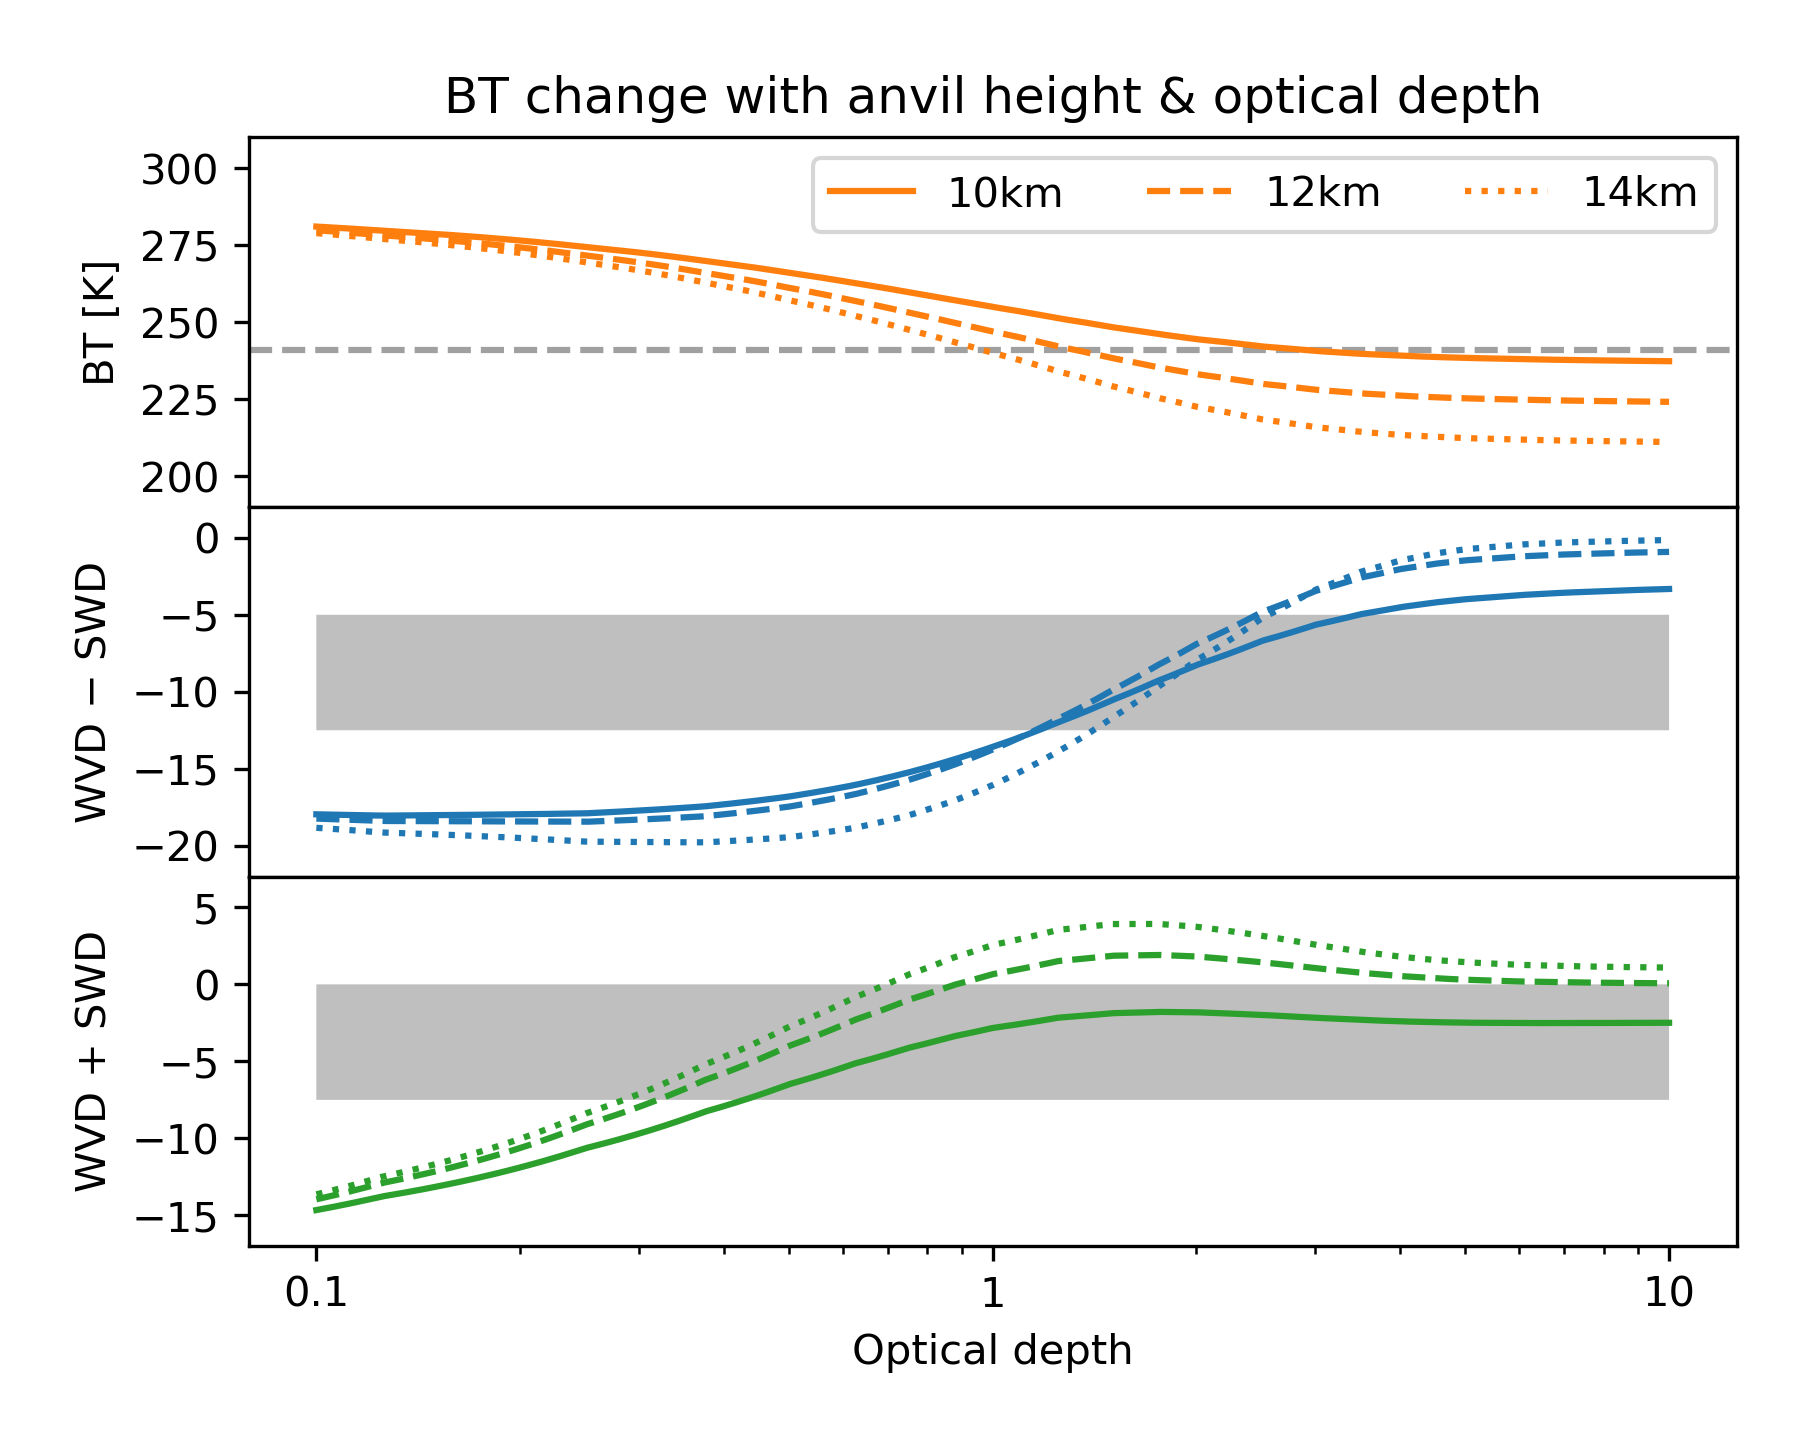
\includegraphics[width=0.9\textwidth]{figures/chapter3_01.png}
    \caption[
    Simulated \acrshort{abi} \acrshort{bt} observations of \acrshort{dcc} anvils at a range of heights and optical depths for detection of thick and thin anvil detection
    ]{
    Simulated \acrshort{abi} \acrshort{bt} observations for \acrshort{dcc} anvils at 10\,\unit{km} (solid lines), 12\,\unit{km} (dashed lines) and 14\,\unit{km} (dotted lines) at optical depths between 0.1 and 10. Panels show (top) 10.4\,\unit{\mu m} \acrshort{bt}; (middle) \acrshort{wvd} minus \acrshort{swd}, used in thick anvil detection; and (bottom) \acrshort{wvd} plus \acrshort{swd}, used in thin anvil detection. The grey dashed line shows the 241\,\unit[K] threshold, and the grey shaded regions show the range in which edge detection is performed for thick and thin anvils.
    }
    \label{fig:bt_wvd_swd_height_od}
\end{figure}

The middle and bottom panels in fig.~\ref{fig:bt_wvd_swd_height_od} show the simulated \acrshort{od} for the combinations of \acrshort{wvd} minus \acrshort{swd} and \acrshort{wvd} plus \acrshort{swd} respectively.
The use of these two combinations for the detection of thick and thin anvil was described in section~\ref{sec:anvil_detection}.
In both panels, the grey shaded region shows the \acrshort{bt} range in which edge detection is used to find the anvil area.
Compared to 10.4\,\unit{\mu m} \acrshort{bt}, the \acrshort{wvd} minus \acrshort{swd} combination shows very little variance in the optical depths at which the anvil cloud is detected within the threshold range.
Throughout the threshold range of --5 to --12.5\,\unit{K} the \acrshort{od} corresponding to the same observed \acrshort{bt} difference varies by approximately 0.1--0.2 between differing heights, compared to 1--2 for 10.4\,\unit{\mu m} \acrshort{bt}.

The \acrshort{wvd} plus \acrshort{swd} combination, shown in the bottom panel of fig.~\ref{fig:bt_wvd_swd_height_od}.
Greater variance between different heights is seen, particularly for the 10\,\unit{km} anvil simulation.
However, the \acrshort{od} corresponding to the observed \acrshort{bt} differences are very similar throughout the detection range of 0 to --7.5\,\unit{K} for heights of 12 and 14\,\unit{km}.
Lidar observations of thin cirrus anvil have shown that the heights of these clouds typically exceed 12\,\unit{km} \citep{wall_observational_2020, horner_evolution_2023}, and so we expect there to be little difference in the sensitivity to most observed anvils.

It should be noted that the simulations shown in fig.~\ref{fig:bt_wvd_swd_height_od} were calculated using a standard tropical atmospheric profile to best represent the moist environment in which deep convection occurs.
While anvils occurring in the extra-tropical parts of the \acrshort{conus} domain are expected to have lower cloud top heights, there is also expected to be a colder temperature profile.
As a result, we expect that the observed \acrshort{bt} for extra-tropical \acrshort{dcc}s behave more like that of the 12 and 14\,\unit{km} simulations shown in fig.~\ref{fig:bt_wvd_swd_height_od}, rather than that at 10\,\unit{km}.

The use of 



\subsection{Estimation of convective intensity and organisation}


\subsection{Lifecycle analysis} \label{sec:lifecycle_definition}

\begin{figure}[tp]
    \centering
    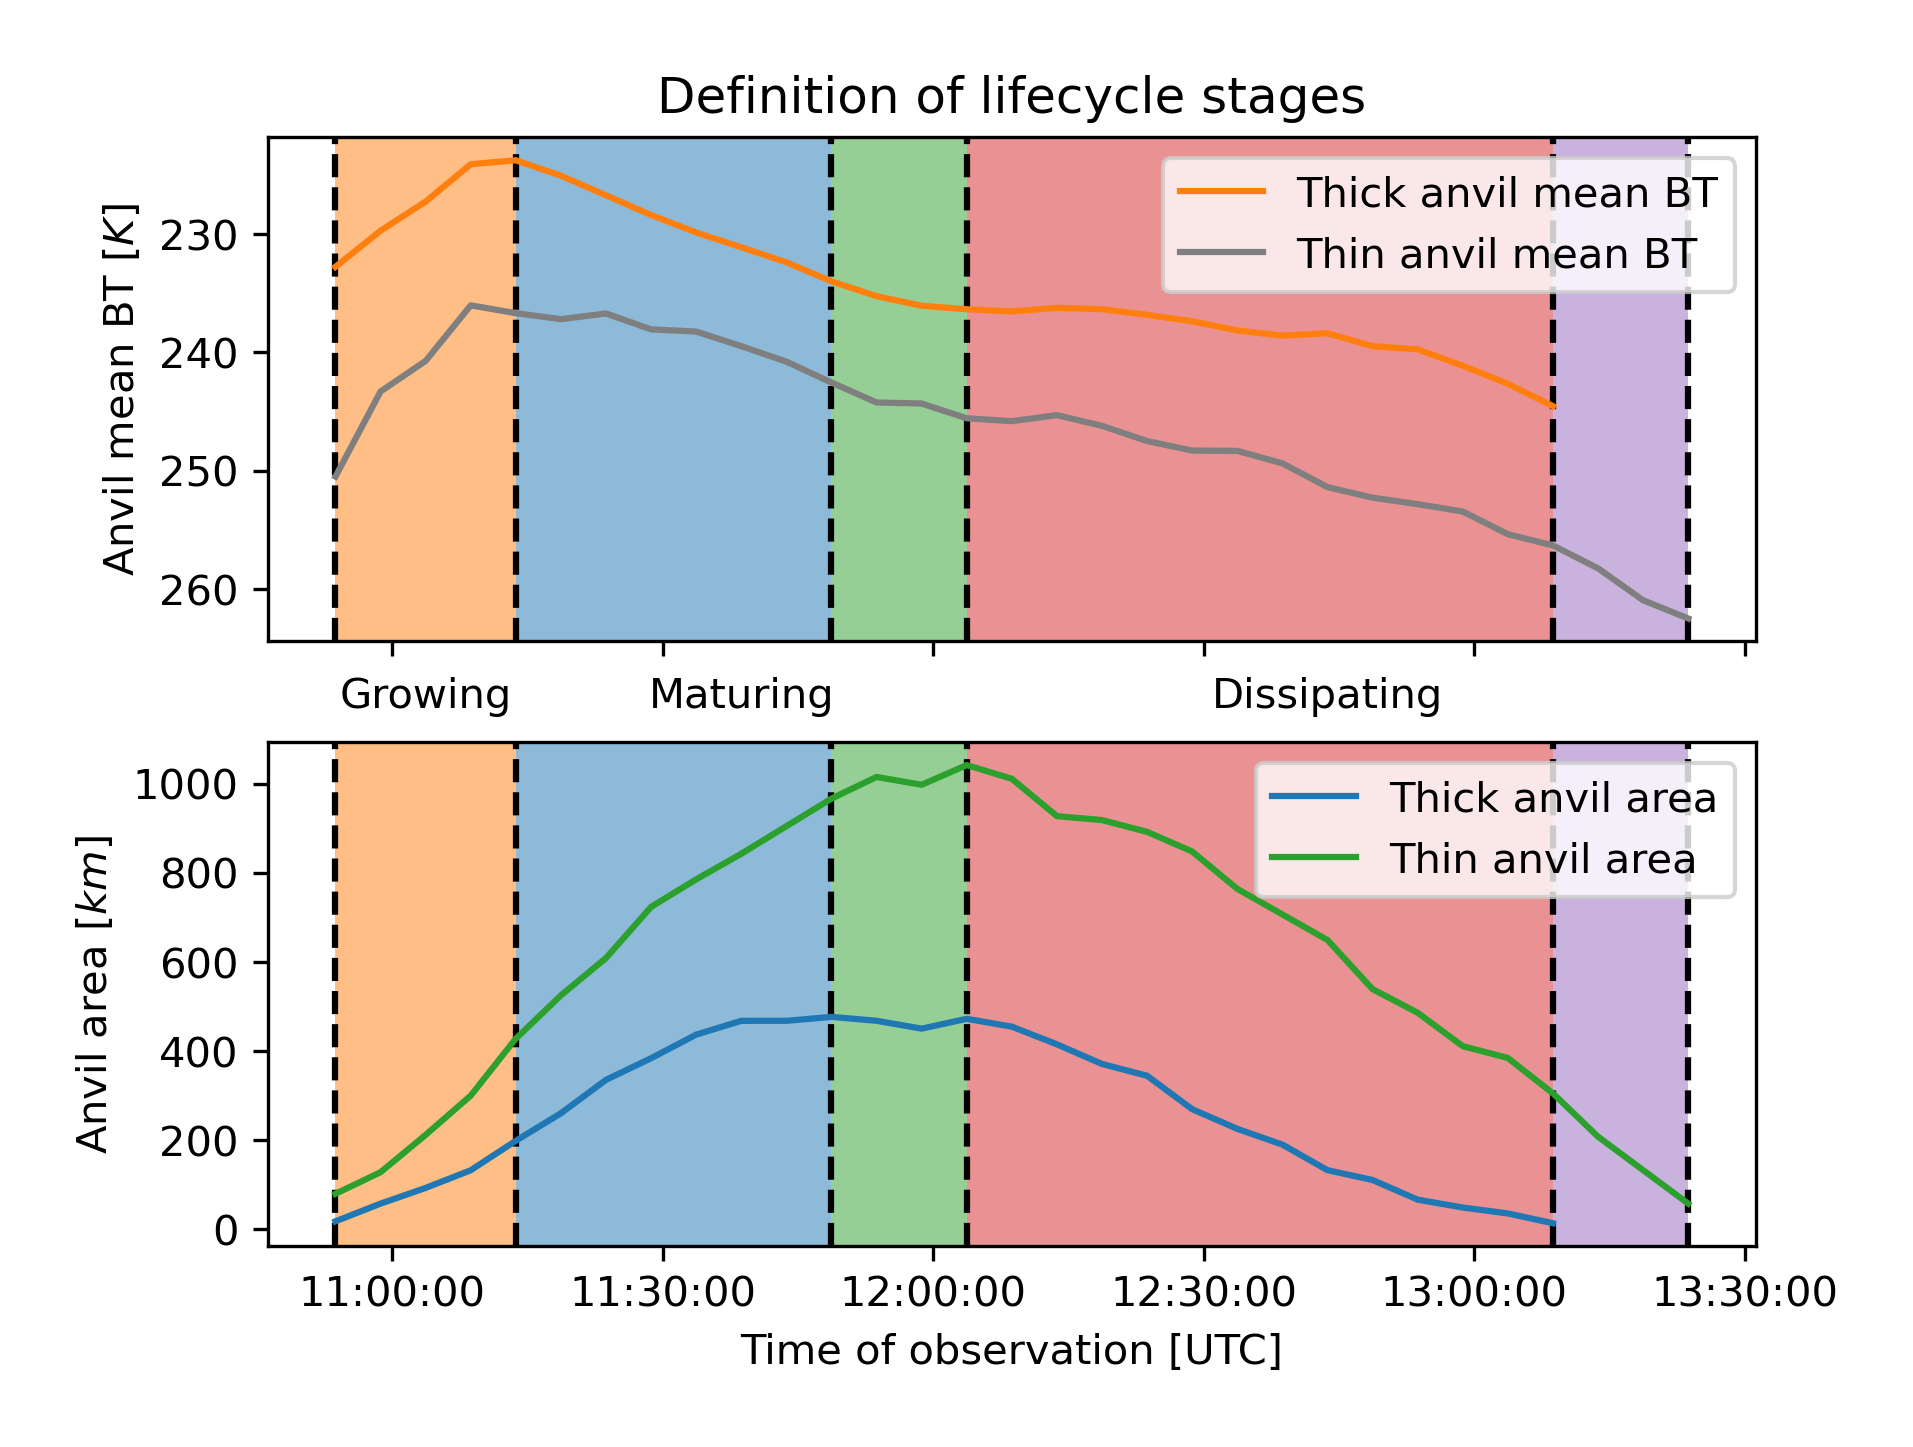
\includegraphics[width=\textwidth]{figures/chapter3_02.png}
    \caption[
    Definition of anvil lifecycle stages based on the method of \citet{futyan_deep_2007}
    ]{
    Definition of anvil lifecycle stages based on the method of \citet{futyan_deep_2007}. The top panel shows the evolution of the mean \acrshort{bt} of the thick and thin anvil regions over the \acrshort{dcc} lifecycle, and the bottom panel shows the evolution of the anvil area. The growing phase (orange) is defined as the time between initial detection and the minimum observed \acrshort{bt}. The mature phase for the thick (blue) and thin (green) anvil is defined as the time between the minimum \acrshort{bt} and maximum thick and thin anvil area respectively. The dissipating phase for the thick (red) and thin (purple) anvils is defined as the time between the anvil maximum area and the final time of detection of the thick and thin anvil respectively.
    }
    \label{fig:lifecycle_example}
\end{figure}


To analyse changes in the lifecycle of \acrshort{dcc}s, we categorise their lifetime based on the method developed by \citet{futyan_deep_2007}.
This method separates the anvil cloud into growing, maturing and dissipating stages based on observations of \acrshort{bt} and anvil area.
\citeauthor{futyan_deep_2007}'s method defines the end of the growing phase as the time at which the anvil reaches its minimum observed \acrshort{bt}, and the end of the mature phase as the time at which the anvil reaches the maximum observed area.
While simple, this approach is applicable to a wide range of observed \acrshort{dcc}s including both isolated and organised convection.
Furthermore, by determining the anvil lifecycle only in terms of the observed anvil properties, we can treat the properties of the detected cores as independent variables allowing straightforward analysis of their impacts on lifecycle.



\section{Results}

%f
\begin{figure}[tp]
    \centering
    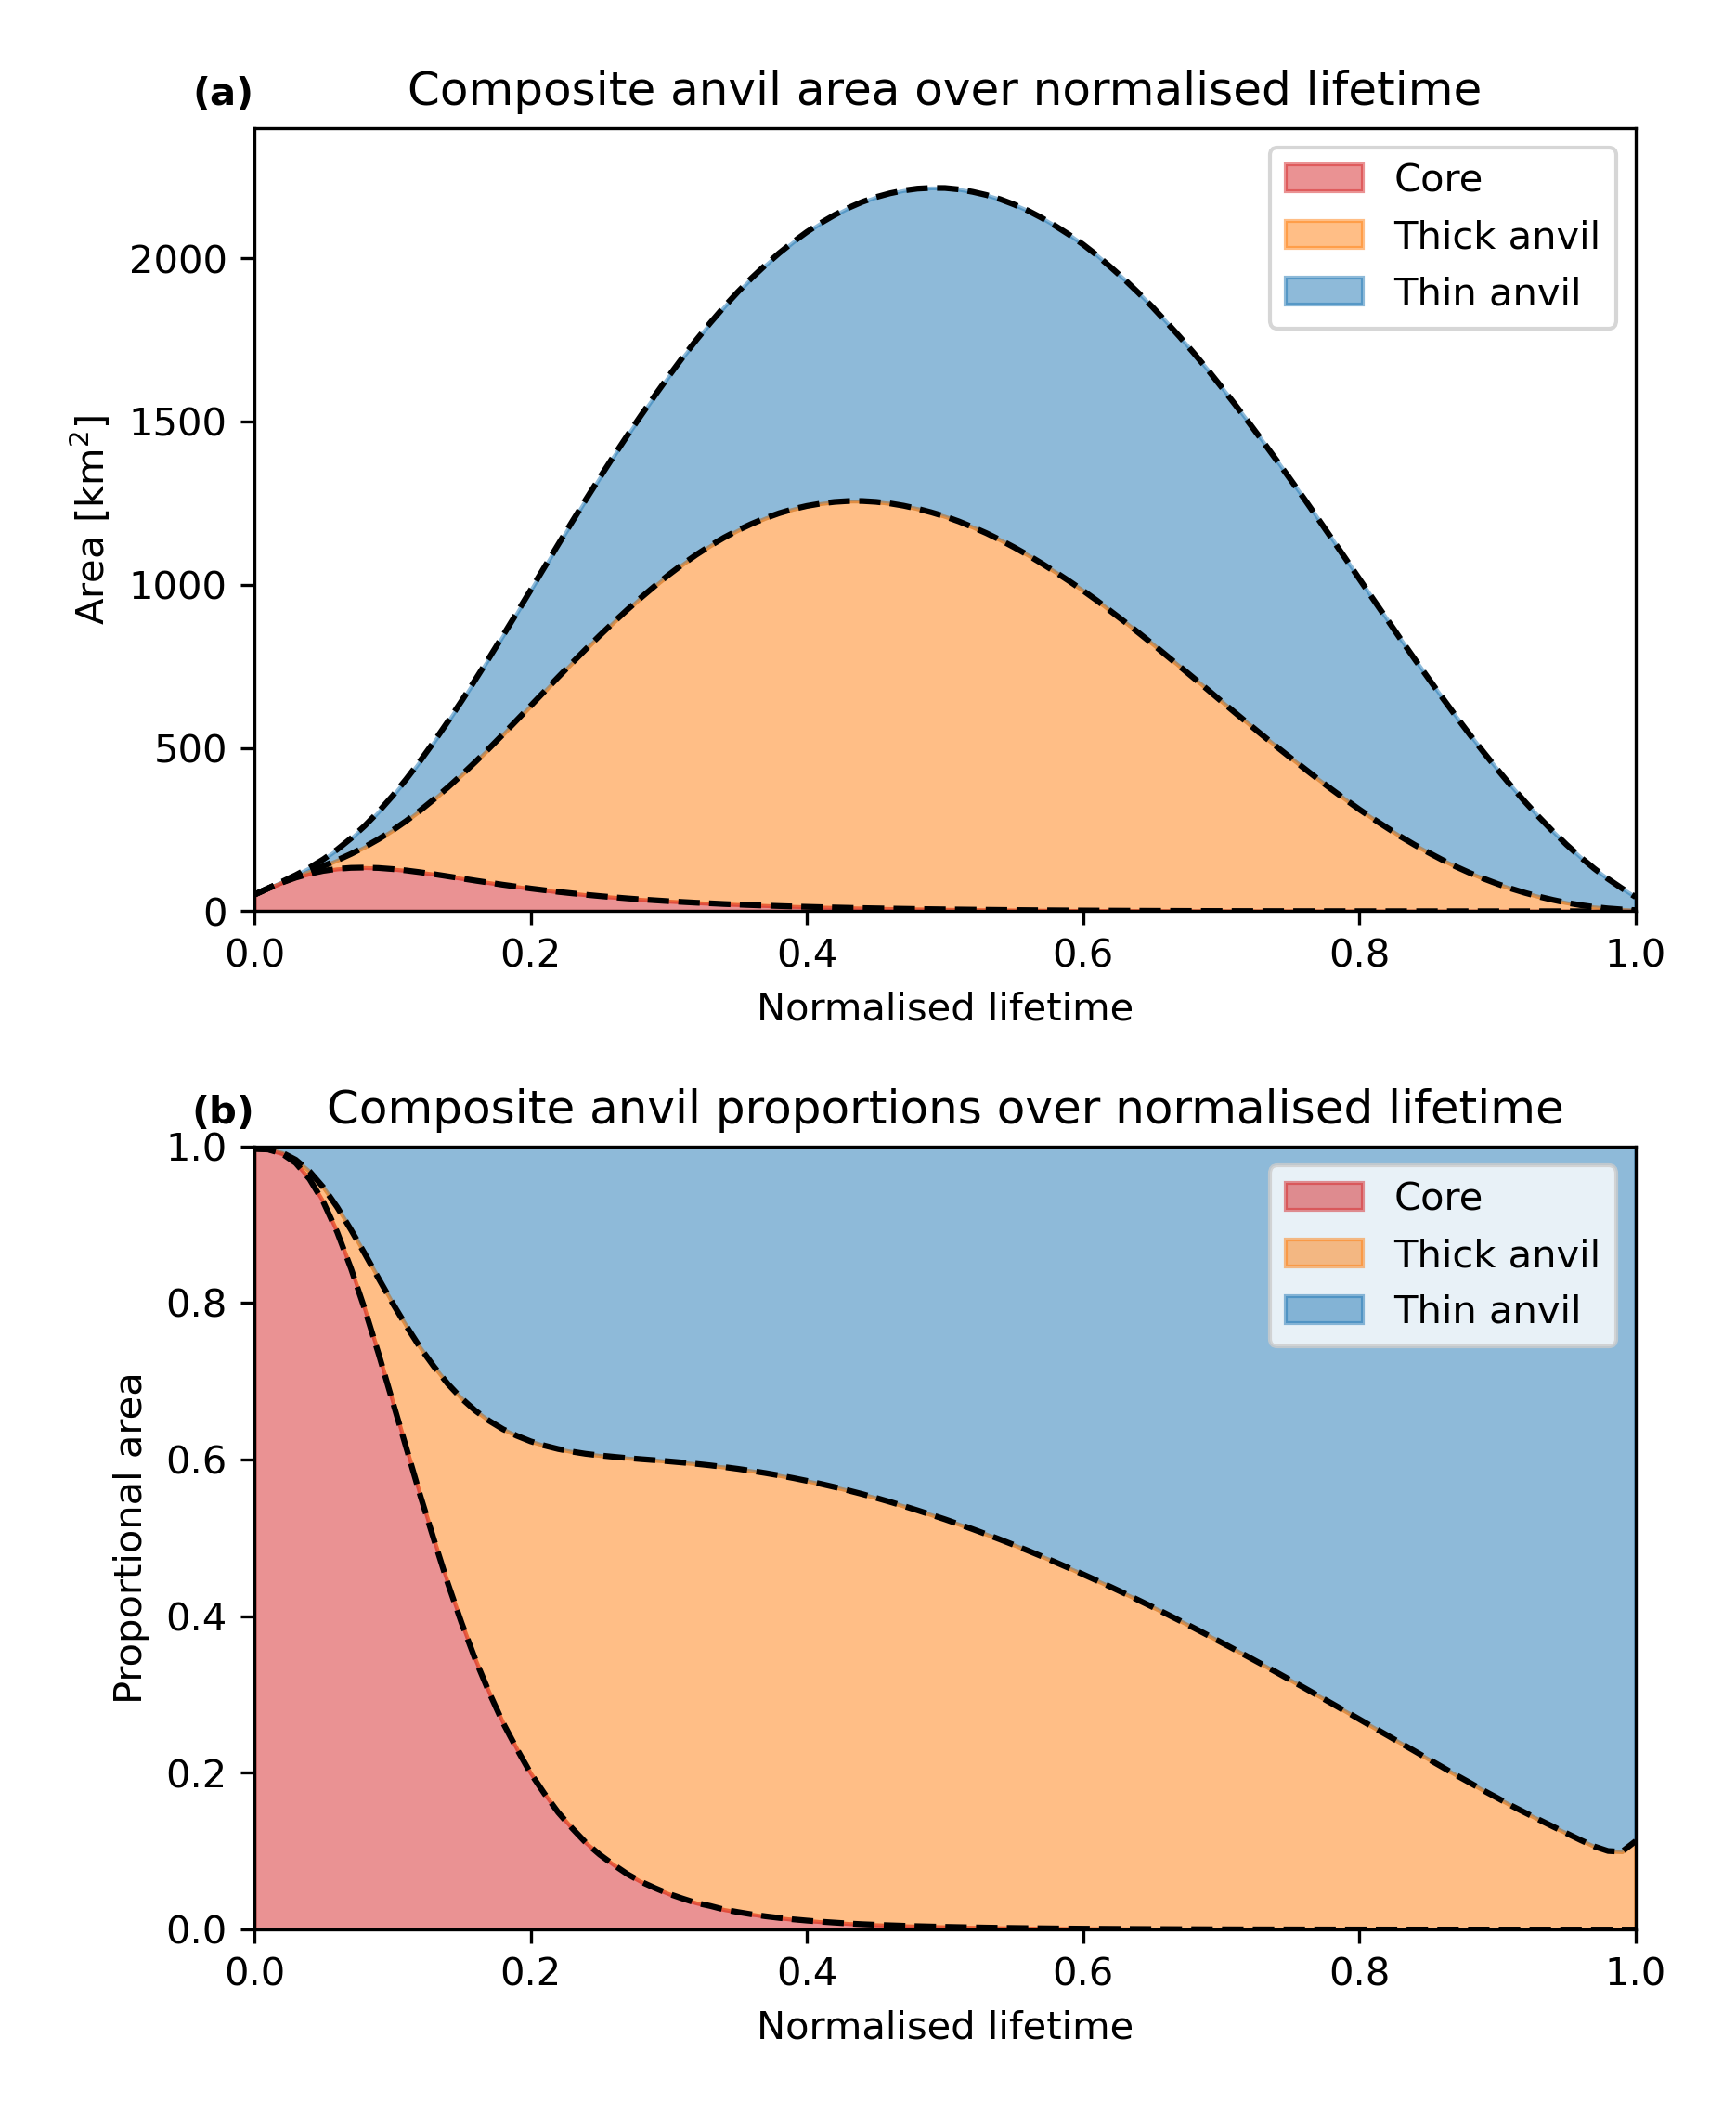
\includegraphics[width=0.75\textwidth]{figures/chapter3_03.png}
    \caption[
    Thin anvil proportion of anvils categorised by mean anvil \acrshort{bt}, initial core cooling rate and number of cores
    ]{
    Thin anvil proportion of anvils categorised by (a) mean anvil \acrshort{bt}, (b) initial core cooling rate, and (c) number of cores. Black error bars show the standard error of the mean, and coloured error bars show the standard deviation.
    }
    \label{fig:thin_anvil_proportion}
\end{figure}

Figure~\ref{fig:thin_anvil_proportion} shows how the observed thin area proportion of observed anvils changes in regard to observed \acrshort{dcc} properties.
In fig.~\ref{fig:thin_anvil_proportion}\,a we show how the thin anvil proportion changes with the average thick anvil \acrshort{bt} (note here that we only consider the thick anvil \acrshort{bt} to avoid a dependence between the anvil \acrshort{bt} and the thin anvil area).
We see an increase of thin anvil proportion with the average anvil \acrshort{bt}, agreeing with the results of \citet{protopapadaki_upper_2017}.
We see a larger thin anvil fraction compared to \citet{protopapadaki_upper_2017} due to observing the lifetime effects on the thin anvil, rather than comparing a single snapshot of anvil area.

Figure~\ref{fig:thin_anvil_proportion}\,b compares how the thin anvil fraction changes with the maximum cooling rate of the initial core associated with the anvil.
Here we see again that there is a positive relation between the strength of convection and the thin anvil fraction.
This also agrees with the results of \citet{takahashi_relationships_2017}, who used radar measurements of convective cores to assess the convective strength and its relationship with thin anvil area.

In fig.~\ref{fig:thin_anvil_proportion}\,c, we compare the thin anvil fraction to the number of cores associated with each anvil.
In contrast to fig.~\ref{fig:thin_anvil_proportion}\,b and c, we see a decrease in the thin anvil fraction with an increase in the number of cores.
As this occurs despite the tendency for multiple-core anvils to have colder average \acrshort{bt}, this indicates that further factors are involved in the thin anvil fraction.

In the rest of this section, we will investigate how both the core intensity and organisation impact the lifecycle anvil clouds, and how these changes influence the thin anvil fraction.

\subsection{Impact of intensity on anvil structure and lifetime}

%f
\begin{figure}[tp]
    \centering
    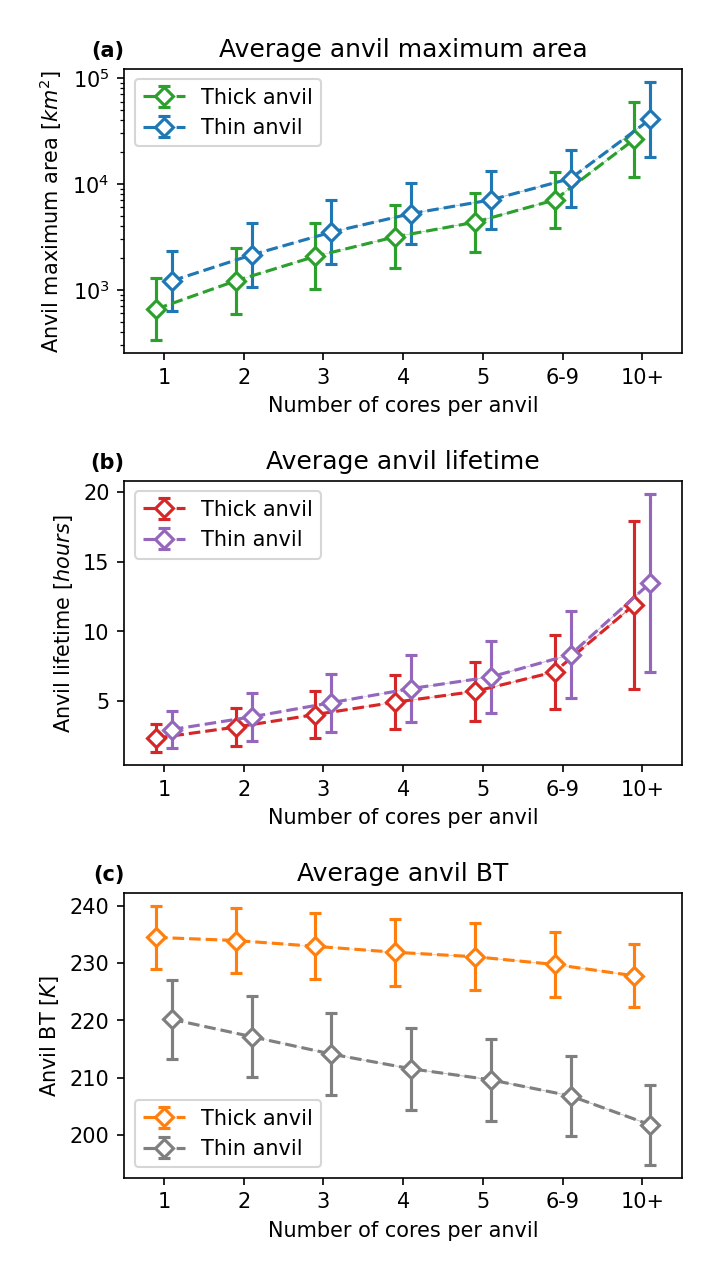
\includegraphics[width=0.75\textwidth]{figures/chapter3_04.png}
    \caption[
    The effect of initial core cooling rate on maximum anvil area, anvil lifetime, and mean and minimum \acrshort{bt}
    ]{
    The effect of initial core cooling rate on (a) maximum anvil area, (b) anvil lifetime, and (c) mean and minimum \acrshort{bt}. Error bars show the standard deviation. Points have been staggered to show the thick and thin anvil properties more clearly, but correspond to the same tick marks on the x axis.
    }
    \label{fig:anvil_cooling_rate_properties}
\end{figure}

%f
\begin{figure}[tp]
    \centering
    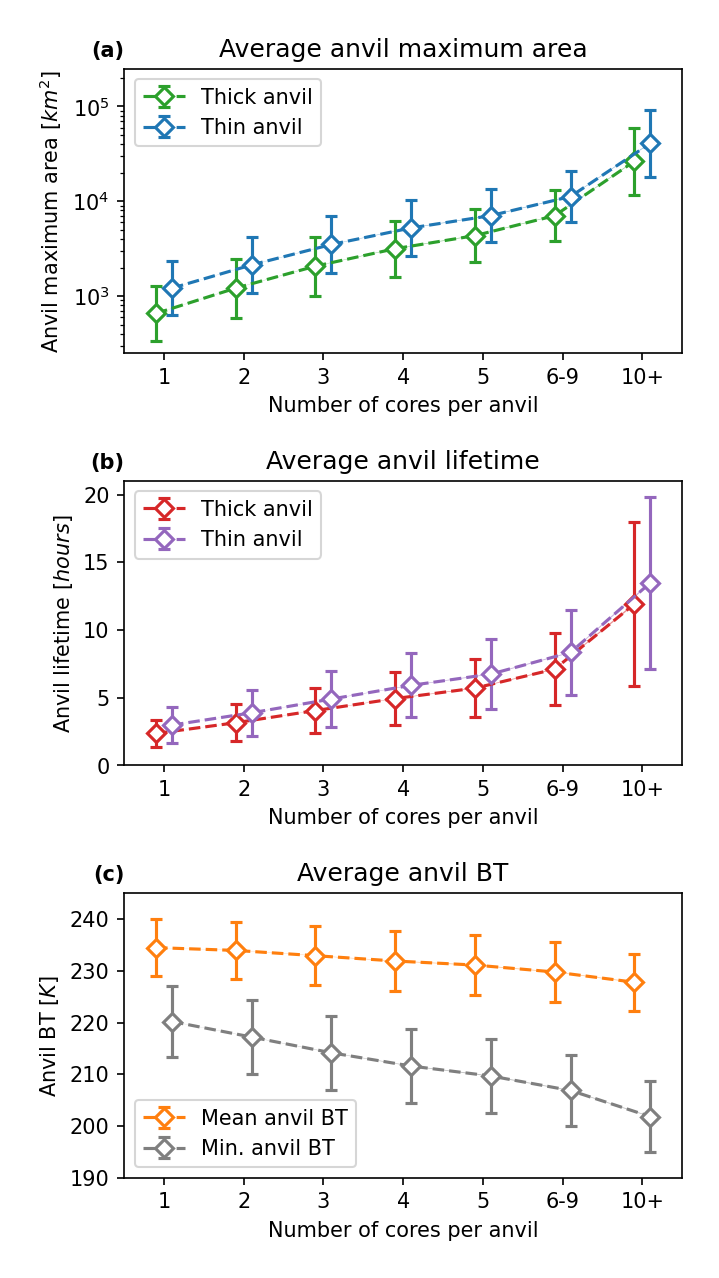
\includegraphics[width=0.75\textwidth]{figures/chapter3_05.png}
    \caption[
    The effect of the number of cores on maximum anvil area, anvil lifetime, and mean and minimum \acrshort{bt}
    ]{
    The effect of the number of cores on (a) maximum anvil area, (b) anvil lifetime, and (c) mean and minimum \acrshort{bt}. Error bars show the standard deviation. Points have been staggered to show the thick and thin anvil properties more clearly, but correspond to the same tick marks on the x axis.
    }
    \label{fig:anvil_number_of_cores_properties}
\end{figure}

We begin by investigating how the properties of observed anvil clouds change with the maximum cooling rate of their initiating core (that is, the first core observed associated with each anvil).
Figure~\ref{fig:anvil_cooling_rate_properties}\,a shows that the average thick and thin anvil maximum areas vary very little with cooling rate, except for at the highest observed values of cooling rate.
There is however a slight widening in the gap between thick and thin anvil maximum area with increasing core cooling rate.
Figure~\ref{fig:anvil_cooling_rate_properties}\,b shows that while the average thick anvil lifetime remains constant with increasing core cooling rate, the thin anvil lifetime increases.
We also see a consistent decrease in both average and minimum thick anvil \acrshort{bt} with cooling rate, shown in fig.~\ref{fig:anvil_cooling_rate_properties}\,c.


%f
\begin{figure}[tp]
    \centering
    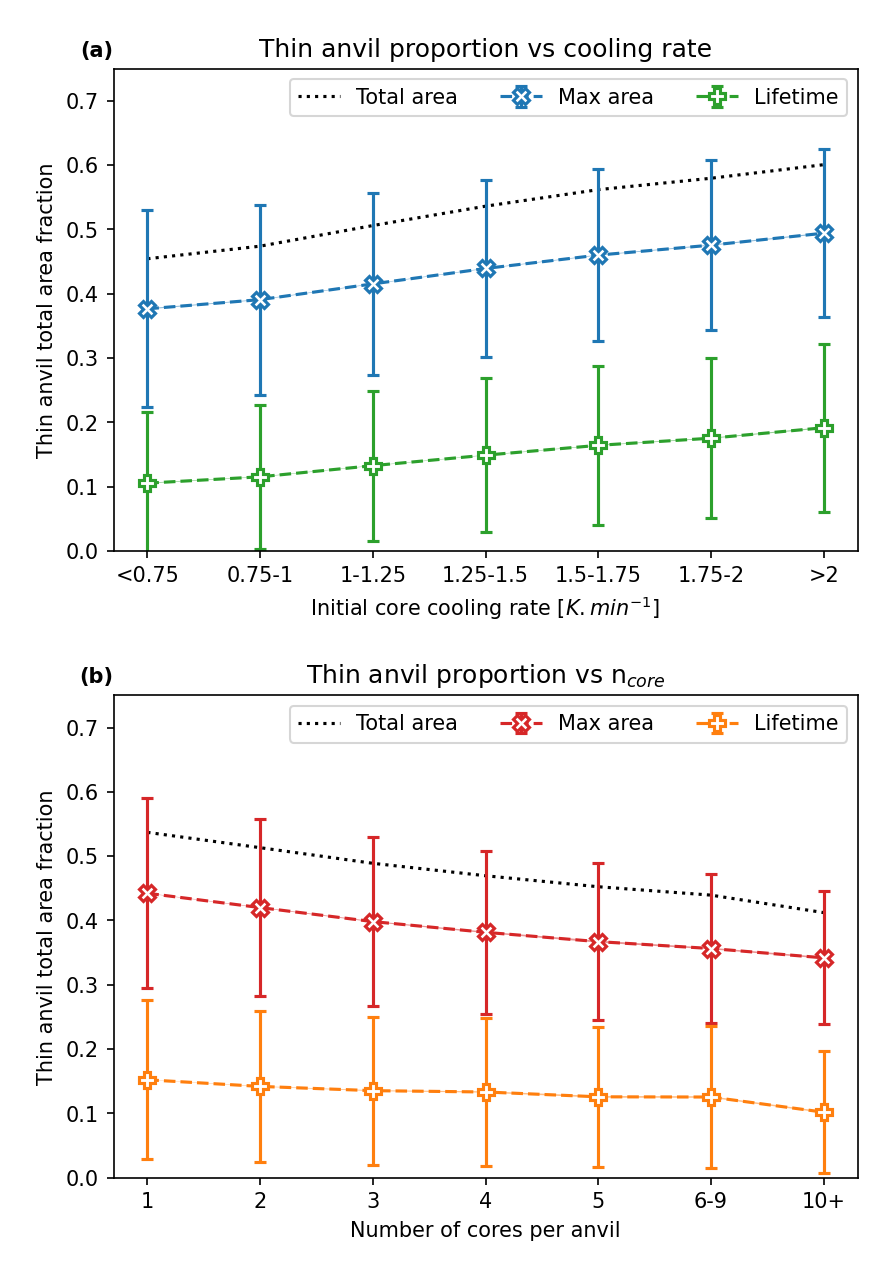
\includegraphics[width=\textwidth]{figures/chapter3_06.png}
    \caption[
    Distributions of anvil lifecycle binned by initial cooling rate
    ]{
    Distributions of anvil lifecycle binned by initial cooling rate. The vertical lines show the mean value of each distribution.
    }
    \label{fig:anvil_cooling_rate_lifecycle}
\end{figure}

Figure~\ref{fig:anvil_cooling_rate_lifecycle} shows the distribution of the different stages of anvil lifecycle for different bins of initial core cooling rate.
With increasing cooling rate the time of coldest mean \acrshort{bt} becomes earlier, mirroring the findings regarding the relationship between core lifetime and cooling rate found in fig.~\ref{fig:core_cooling_rate_relations}.
While the timing of the maximum thick anvil area and thick anvil dissipation show little change with cooling rate, the time of thin anvil maximum area and dissipation increase.


%f
\begin{figure}[tp]
    \centering
    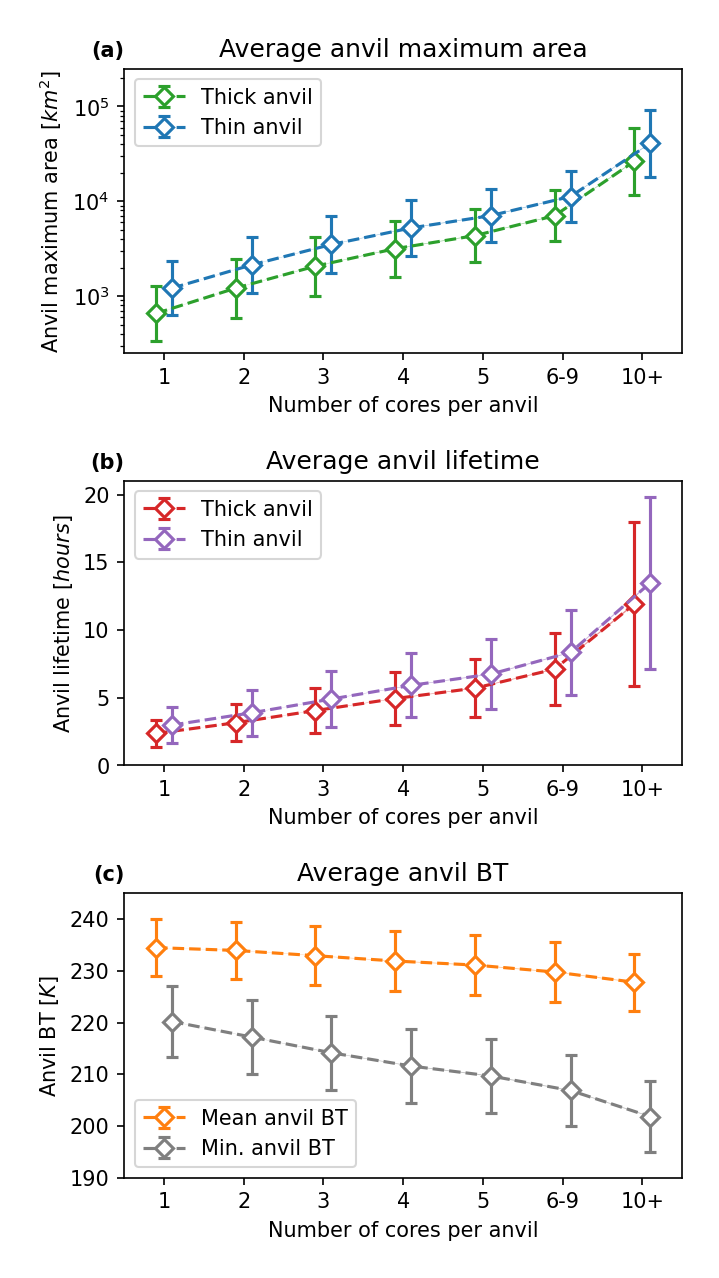
\includegraphics[width=\textwidth]{figures/chapter3_07.png}
    \caption[
    The average fraction of anvil lifetime of each lifecycle stage for anvils categorised by initial core cooling rate
    ]{
    The average fraction of anvil lifetime of each of the lifecycle stages defined in section~\ref{sec:lifecycle_definition} for anvils categorised by initial core cooling rate. Each bar is normalised such that the total length of the row is equal to the mean thin anvil lifetime of its cooling rate bin.
    }
    \label{fig:anvil_cooling_rate_proportional_lifecycle}
\end{figure}

Figure~\ref{fig:anvil_cooling_rate_proportional_lifecycle} displays the average proportion of anvil lifecycle spent in each of the stages shown in fig.~\ref{fig:anvil_cooling_rate_lifecycle}.
We see again that the primary effect of core cooling rate is to reduce the growing phase and increase the thin anvil dissipation stage.
The thick anvil mature stage remains similar across cooling rate, as does the time between the thick anvil maximum area and thick anvil dissipation.
Overall, this indicates that core cooling rate primarily affects the thin anvil properties, and that the increase in the proportion of thin anvil with cooling rate  is mostly due to an increase in the thin anvil lifetime.

\subsection{Impact of organisation on anvil structure and lifetime}

In fig.~\ref{fig:anvil_number_of_cores_properties} we examine how the anvil properties change with the number of cores associated with each anvil cloud.
Figure~\ref{fig:anvil_number_of_cores_properties}\,a shows that both the thick and thin anvil maximum area increase substantially with an increasing number of cores.
However, the thin anvil area increases at a slower rate proportional to the thick anvil.
We see a similar increase in the thick and thin anvil lifetime with increasing number of cores in fig.~\ref{fig:anvil_number_of_cores_properties}\,b.

We see a similar rate of the decrease of average anvil \acrshort{bt} with the number of cores in fig.~\ref{fig:anvil_number_of_cores_properties}\,c as we did in relation to core cooling rate in fig.~\ref{fig:anvil_cooling_rate_properties}\,c.
The minimum anvil \acrshort{bt} decreases at a notably faster rate with increasing number of cores however.
Although this is indicative of an increased likelihood of overshooting cores in more organised \acrshort{dcc}s, we must also note that the larger area of these systems also makes it more likely to observe colder pixels.

%f
\begin{figure}[tp]
    \centering
    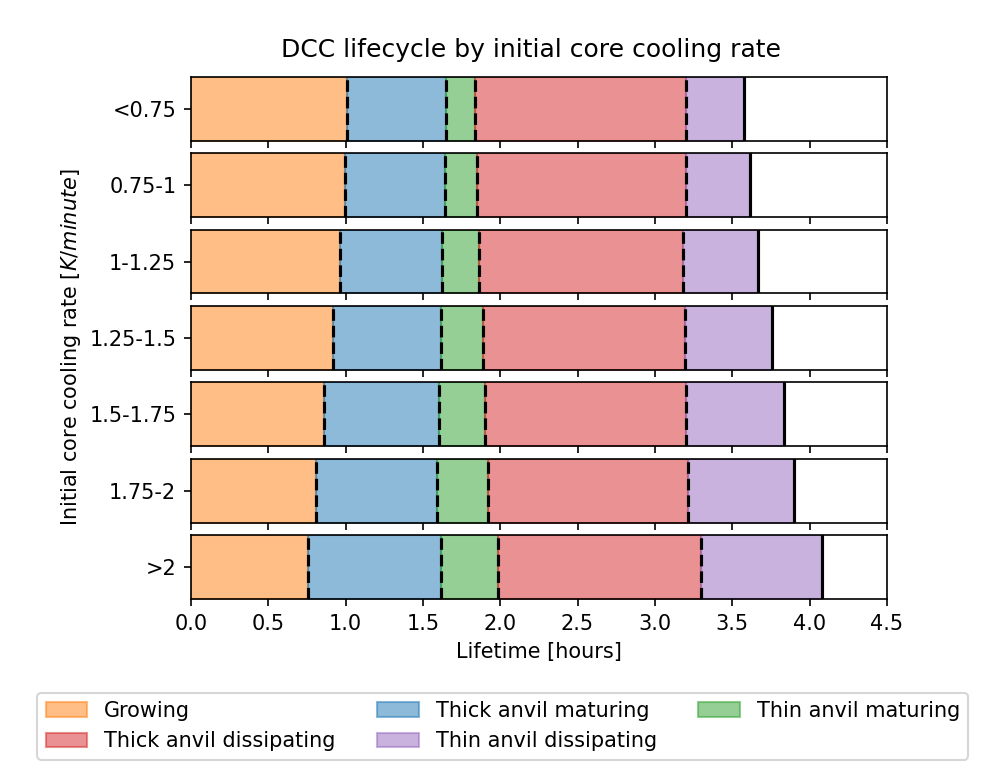
\includegraphics[width=\textwidth]{figures/chapter3_08.png}
    \caption[
    Distributions of anvil lifecycle binned by number of cores
    ]{
    Distributions of anvil lifecycle binned by number of cores. The vertical lines show the mean value of each distribution.
    }
    \label{fig:anvil_number_of_cores_lifecycle}
\end{figure}

Figure~\ref{fig:anvil_number_of_cores_lifecycle} shows how the timing of the different anvil stages changes with increasing number of cores.
In general, the lifetime of every stage of the \acrshort{dcc} lifecycle increases with the number of cores.
However, the time between the thick and thin anvil maximum area and the thick and thin anvil dissipation increase at a slower rate proportion to the lifetimes of those stages.

%f
\begin{figure}[tp]
    \centering
    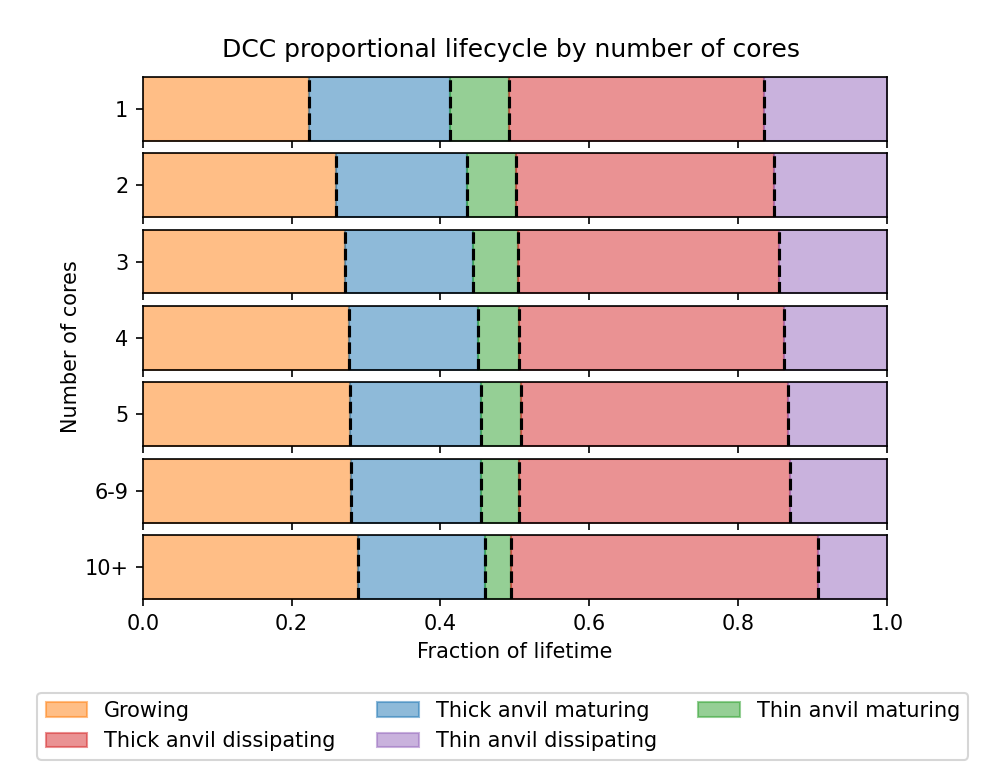
\includegraphics[width=\textwidth]{figures/chapter3_09.png}
    \caption[
    The average fraction of anvil lifetime of each lifecycle stage for anvils categorised by number of cores
    ]{
    The average fraction of anvil lifetime of each of the lifecycle stages defined in section~\ref{sec:lifecycle_definition} for anvils categorised by number of cores. Each bar is normalised such that the total length of the row is equal to the mean thin anvil lifetime of its number of cores bin.
    }
    \label{fig:anvil_number_of_cores_proportional_lifecycle}
\end{figure}

Figure~\ref{fig:anvil_number_of_cores_proportional_lifecycle} shows the proportion of the overall anvil lifetime spent in the different stages for increasing number of cores, similar to that in fig.~\ref{fig:anvil_cooling_rate_proportional_lifecycle}.
Unlike fig.~\ref{fig:anvil_cooling_rate_proportional_lifecycle}, we see an increase in the growing phase with increasing number of cores, and a decrease in the thin anvil dissipation phase.
In addition, while the thick anvil maturing phase changes little with the number of cores, the time for the thin anvil to reach its maximum area is substantially shorter for \acrshort{dcc}s with the most cores.
It is a combination of the smaller proportional increase in area for the thin anvil, seen in fig.~\ref{fig:anvil_number_of_cores_properties}, and smaller proportion of the \acrshort{dcc} lifecycle spent in the thin anvil dissipating phase which account for the reduction in the thin anvil proportion for increasing number of cores seen in fig.~\ref{fig:thin_anvil_proportion}\,c.

\section{Summary}

The most interesting result from this comparison is that while the core intensity and \acrshort{dcc} organisation have similar relations to anvil \acrshort{dcc}---the most common proxy used for convective intensity in satellite studies of \acrshort{dcc}s---the have opposite effects on the anvil lifecycle in relation to the thin anvil cirrus.
While \acrshort{dcc}s with individually stronger cores tend to enhance the area and lifetime of thin anvil cirrus, more organised \acrshort{dcc}s, despite their overall larger area and lifetime, tend to produce a smaller amount of thin anvil in proportion to their thick anvil area.
These two competing effects on thin anvil proportion between two modes of convective intensity may act to control the overall amount of thin anvil cirrus produced by \acrshort{dcc}s.
